\section{Output}
Depending on application, different output formats might come in handy. PET
supports printing plain time power dump, a somewhat more readable table to
plain, table and a gnuplot figure with time as X-axis and power drain on the
Y-axis. The output format is understood as timeslots in which the architecture
has a certain current drain, which should be multiplied with applied voltage to
get numbers on consumed energy, heat generation and so on. The numbers are
scaled as milliamperes, which of course is equal to milliwatt if voltage is
$1V$.

Example of the \texttt{plain} output format can be seen in
\autoref{lst:pet_output_plain}. The left column is the bucket number, while the
right column is instant current draw from the modelled architecture.

\begin{lstlisting}[label={lst:pet_output_plain},caption={PET Plain Output}]
0 120
1 113
2 150
3 123
4 133
5 117
\end{lstlisting}

When reading the output directly from console, a more descriptive output format
is the \texttt{table} format. An example using this option is rendered in
\autoref{lst:pet_output_table}.

\begin{lstlisting}[label={lst:pet_output_table},caption={PET Table Output}]
/-------------------------\
|   Bucket   |   Energy   |
|-------------------------|
|          0 | 120.000000 |
|          1 | 113.000000 |
|          2 | 150.000000 |
|          3 | 123.000000 |
|          4 | 133.000000 |
|          5 | 117.000000 |
\-------------------------/
\end{lstlisting}

Visualization is often a good thing when inspecting old or trying to understand
new problems. As it is hard to get a good overview from huge text log files, PET
provides, as stated in \autoref{subsec:annot}, an optionally annotated graphical
output. In effect, it is formatting temporary output files and calling GNUPlot
do do the hard work.

\begin{figure}
    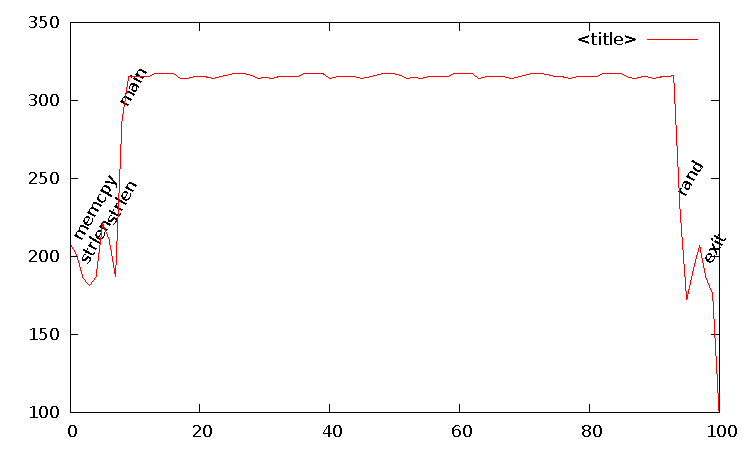
\includegraphics[width=0.9\textwidth]{figs/annot.pdf}
    \caption{PET Annotated Graphical Output}
    \label{fig:annot}
\end{figure}

